\documentclass[12pt,a4paper]{article}

%% fonts
\usepackage{fontspec}
\setromanfont[Mapping=tex-text]{Minion Pro}
\setmonofont{Inconsolata}
\usepackage[normalem]{ulem}

\usepackage[hmargin=2.5cm]{geometry}

%% flexible lists
\usepackage{paralist}

%% more sane tables
\usepackage{booktabs}
\usepackage{longtable}

%% graphics
\usepackage[xdvi]{graphicx}
\usepackage{rotating}

%% add a bit more spacing between paragraphs
\renewcommand{\baselinestretch}{1.1}

%% hyperlinks -- must be last
\usepackage{color}
\usepackage[colorlinks=true,linkcolor=blue,urlcolor=blue]{hyperref}


%% metadata for pdf 
\newcommand{\pdfsubj}{COMP3301\slash COMP7308}
\newcommand{\pdftitle}{Assignment 1 --- User-space scheduler}
\newcommand{\pdfauthor}{John Williams and Sam Kingston}
\newcommand{\assignnum}{a1}
\newcommand{\assignweight}{20\% }
\title{\pdftitle}
\author{\pdfauthor}
\hypersetup{
    pdftitle={\pdftitle},
    pdfauthor={\pdfauthor},
    pdfsubject={\pdfsubj}
}


\newcommand{\duedate}{8pm Thursday 15 September 2011}

\begin{document}

\begin{center}
\large \textbf{The University of Queensland} \\
\large \textbf{School of Information Technology and Electrical Engineering} \\
\large \textbf{Semester Two, 2011}
\end{center}

\begin{center}
\Large \textbf{\pdfsubj} \\
\Large \textbf{\pdftitle}
\end{center}

\begin{center}
\large \textbf{Due: \duedate} \\
\large \textbf{Weighting: \assignweight for COMP3301 students (100 marks total)}
\end{center}


\begin{center}
\color{blue}
Version 1.2 --- 9 September 2011 \\
See Changelog on last page for updates.
\end{center}

\subsection*{Introduction}

The goal of this assignment is to give you a practical knowledge of operating
system schedulers and the experience in modifying them in a defined way.

As part of the assessment you must also answer some short--response questions
that will test your understanding of the concepts that you have implemented.

This assignment may be completed \textbf{individually} or in
\textbf{self-selected groups of two}. Please read the section on group work if
you decide to work in groups of two. Although you may share code with your team
member (if working in groups of two), it is still considered cheating to look
at another student's code or allow your code to be seen or copied. You should
be aware that all code submitted may be subject to automated checks by
plagiarism-detection software.  You should read and understand the school's
policy on student misconduct, which is available at:
\url{http://www.itee.uq.edu.au/about_ITEE/policies/student-misconduct.html}.

\subsection*{Pth---GNU Portable Threads}

Pth is a portable userland threading library that can be linked against to
provide threading capabilities to a process. You should be familiar with this
library from the practicals. It is suggested you review these before starting
the assignment.

The default Pth scheduler operates in a cooperative manner --- threads must
yield the CPU for other threads to run. Pth has been modified for you to
include a preemptive scheduler, that can interrupt a thread if it runs longer
than the fixed scheduling quantum. All further references to Pth refer to this
preemptive version, and you will complete this assignment using that version.
You may download Preemptive Pth from the course website. Do not download from any
other source, as this will be the unmodified version.

\subsection*{Scheduling behaviour}

The current Pth scheduler implements a round-robin algorithm where each thread
is given a time slice to run in turn. If the thread does not yield by the end
of this fixed time slice then it is preempted, and the next ready thread is
run. It does not provide any mechanism for a thread to specify a deadline.

Your task is to modify the Pth scheduler to implement the \textbf{earliest
deadline first} scheduling algorithm. You should be familiar with this
algorithm from lectures, so refer to the corresponding lecture notes if you need more
information. The new algorithm will replace the current round-robin one.

Threads will specify their deadline on creation through two new attributes:
\texttt{PTH\_ATTR\_DEADLINE\_C} (execution time) and
\texttt{PTH\_ATTR\_DEADLINE\_T} (period). Both deadlines are strictly positive
integer {\color{blue}multiples of the time slice} (that is, both are strictly $> 0$). You must create these new
attributes and expose them through \texttt{pth.h} (hint: do not add these directly
to \texttt{pth.h} as this is automatically generated). Ensure you can set and get
the attributes from a test program. For instance, a thread may specify its
deadline as follows:

\texttt{PTH\_ATTR\_DEADLINE\_C} $= 1$

\texttt{PTH\_ATTR\_DEADLINE\_T} $= 5$

{\color{blue}The above example means that a thread has a deadline of once every 5 time slices.}

New threads should inherit the deadlines of their parent threads, but may be
overridden by calls to \texttt{pth\_attr\_set()}. If not specified (and not
inherited), the attributes should default to the following:

\begin{longtable}{l l}
    \toprule
    \texttt{PTH\_ATTR\_DEADLINE\_C} & $1$ \\
    \texttt{PTH\_ATTR\_DEADLINE\_T} & $10$ \\
    \bottomrule
\end{longtable}

When creating a thread, the scheduler should validate the deadline attributes
and see if the system is still schedulable with the addition of the new thread.
If either of these conditions fail, the scheduler must deny the thread's
creation (by returning the error specified below). {\color{blue}You do not have to
handle the case where a thread's deadline is not an integer multiple of the time slice.} Recall that the
schedulability test of earliest deadline first is:

\begin{displaymath}
\sum_{i=1}^{n} \frac{C_i}{T_i} \leq 1
\end{displaymath}

On each scheduling decision, the thread with the earliest deadline should be
run. If a clear decision cannot be made, the system should enter a tie break as
follows:

\begin{compactenum}
    \item If one of the tied threads ran in the last scheduling period,
    continue running it (see figure 1 for an example)
    \item If neither thread ran in the last scheduling period, pick the oldest
    thread
\end{compactenum}

Once a thread has reached its deadline, it should be removed from consideration until
the next multiple of its deadline is reached. For instance a thread specifying a deadline
of once every 5 seconds will be runnable at $t=0$, $t=5{\color{blue}00}$, $t=1{\color{blue}000}$, \textit{etc.} {\color{blue}(where $t$ is in milliseconds.)}

For simplicity, if a thread yields via \texttt{pth\_yield()} or otherwise makes
a call into Pth's {\color{blue}POSIX replacement} library {\color{blue}(e.g. \texttt{write(2)})}, you can consider it finished for the current
scheduling slice and the scheduler should enter an idle loop until the next
scheduling slice. {\color{blue}\sout{Do not spin the CPU here; it may be sufficient to sleep for a
fixed period}} (it is up to you to decide how to handle this edge case).

You should ensure that you do not disrupt Pth's event handling mechanism or its
queue management functions (such as moving a thread between priority queues).
You may be tested on simple events (such as thread I\slash O, sleeping).

\subsection*{Sample thread system}

The following sample thread system are provided so you can visualise the
concepts and behaviour specified. Note that it is a simplified and contrived
example. The scheduling period is shown as 1 second, whereas the Pth period is
100 ms.

\begin{figure}[htb]
    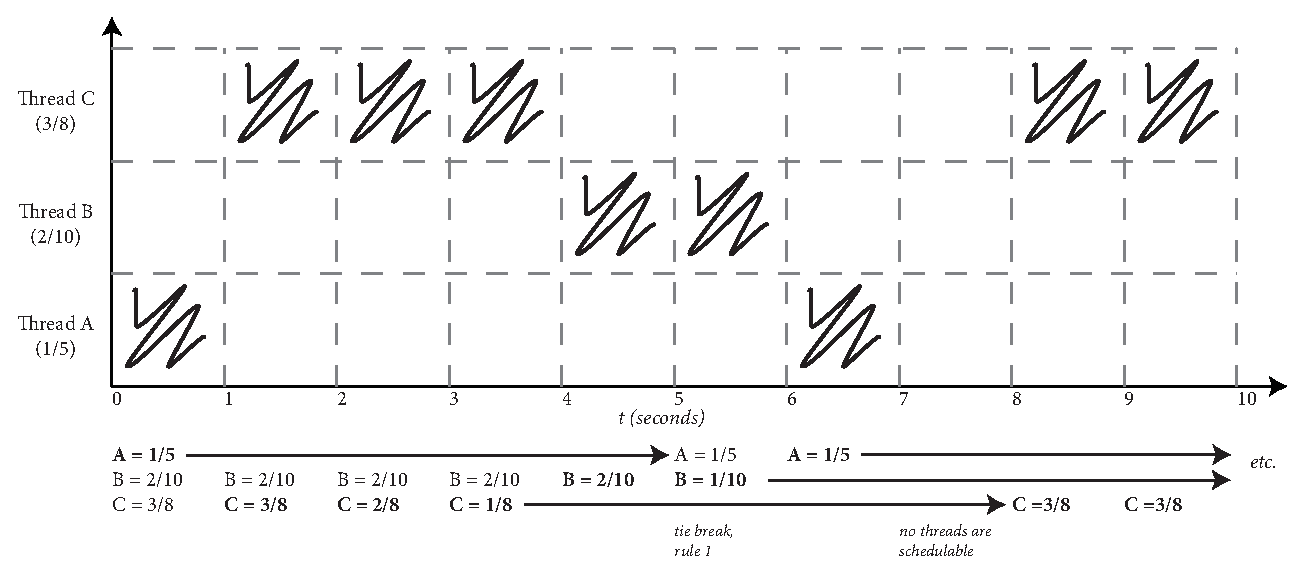
\includegraphics[scale=0.75]{example-system1.eps}
    \caption{Sample thread system where scheduling period is 1 second}
    \label{sample1}
\end{figure}

\subsection*{Thread creation errors}

Some additional errors may be returned if a new thread cannot be created. These
should be returned via the \texttt{pth\_error} function.

\begin{longtable}{l l}
    \toprule
    \textbf{\texttt{errno} code} & \textbf{Reason for error} \\
    \midrule
    \texttt{ERANGE} & if \texttt{PTH\_ATTR\_DEADLINE\_C} $>$ \texttt{PTH\_ATTR\_DEADLINE\_T} \\
    \texttt{EAGAIN} & if schedulability test fails \\
    \bottomrule
\end{longtable}

\subsection*{Scheduling logging}

As part of the assignment, you must also modify the Pth scheduler to output a log
file with information on each thread's running time, as shown below. The output
must be exactly as described as it will be automatically marked. This logging
will give a visual representation of the scheduling decisions your scheduler is
making, such as the order in which threads are picked, and how long they run
for. It may be useful to start the assignment with this logging.

The behaviour of this logging is as follows:

On initialisation, the scheduler shall open a file called \texttt{sched.log} in
the current working directory. If an existing file by this name exists, it
should be overridden. Any errors in opening the file (such as permissions)
should cause the initialisation to fail and a descriptive error to be printed
to \textit{standard error} (consider using \texttt{perror(3)}). {\color{red}\sout{After
successful opening,} Each time a user-created thread is created,} a header row will be written to the file in the following
format (followed by a newline):

\verb|t       |$T_i$\verb|     |$T_{i+1}$\verb|  |\dots\verb|  |$T_n$

where $T_i$ is the name of the first {\color{blue}user-created} thread, $T_{i+1}$ is each consecutive
thread (if any), up to the last thread, $T_n$. Each column should be padded to
8 spaces, with at least one space between each (you may wish to consider using
the \texttt{printf} padding specifier for this). Therefore if a thread name is
longer than 7 characters, it should be truncated (7 visible characters and 1
space make up each column heading).  There should be no leading or trailing
spaces on any line, nor should there be any blank lines. The order of columns
should be in order of thread creation, and should never change order. Do not
include the scheduler or main threads. For example, a valid header row may be:

\begin{verbatim}
t       nice    greedy
\end{verbatim}

Every time a new {\color{blue}user-created} thread is created, the header row should be updated and
written to the file again. For example, adding a new thread  to the above
example may cause the following header row to
be written:

\begin{verbatim}
t       nice    greedy  greedy2
\end{verbatim}

If multiple threads are created before any run, then multiple header rows will
be present in the log file.

For every scheduling decision, the time since epoch (rounded to the nearest
whole millisecond) of when the thread started running should be written in the
first column (under \texttt{t}), padded to 8 spaces. Note that this means if
a thread yields in under 1 millisecond, the start time of it and the next thread
will be the same. This is expected behaviour. For the purposes of this
assignment, the epoch should be fixed to when the first {\color{blue} user-created} thread begins running
{\color{blue}\sout{(note this may not be the first \textit{user-created} thread)}}.

Three \texttt{+} characters should then be written in the corresponding column
for the thread that just ran, directly followed by a \texttt{P} if the thread
was preempted, or a \texttt{Y} if the thread yielded.  See
{\color{red}\sout{below} above at the bottom of the ``Scheduling behaviour''
section} for information on threads yielding.

{\color{red}If no thread ran in the given period (see Figure 1 at $t=7$ for instance),
the written line should only contain the time since epoch.}

You will need to make sure you insert enough padding so the first character of
the \texttt{+} lines up with the first character of the thread's name in the
header row. For example, assuming the threads in the above example were
all started in the main function, a possible log file output may be:

\begin{verbatim}
t       nice    greedy  greedy2
0       +++Y
0               +++P
100                     +++P
200             +++P
300                     +++P
400     +++Y
t       nice    greedy  greedy2 greedy3
400                             +++P
\end{verbatim}

This output (assumed complete) reveals the following about the test program:

\begin{itemize}
    \item The order of running was: \texttt{nice}, \texttt{greedy},
    \texttt{greedy2}, \texttt{greedy}, \texttt{greedy2} and \texttt{nice}

    \item The \texttt{nice} thread yielded cooperatively back to the scheduler
    in under 1 millisecond

    \item The greedy threads were preempted after 100 milliseconds each, which
    reveals that the scheduling time slice is set to 100 milliseconds

    \item The \texttt{nice} thread was either waiting on an event or sleeping
    for at least 1 second

    \item At approximately 400 milliseconds since program start a new thread
    \texttt{greedy3} was created

    \item The program exited after the \texttt{greedy3} thread was preempted,
    which based on previous observations can be computed to half a second after
    the first thread was run

    \item {\color{red}The scheduler used to produce these outputs implements the round-robin algorithm,
    \textbf{not} the algorithm specified in this assignment}
\end{itemize}

You should try to print log outputs as ``close'' to scheduling decisions as
possible to ensure scheduling overhead does not creep into the time column (for
instance if the scheduler spends 5 milliseconds doing housekeeping after a
thread returns but before writing to the log file, you should ensure this 5
milliseconds isn't included in the time column).

It is expected that you may see some small drift in the times for a long
running program due to factors outside of your control, however each time slice
should always be 100 milliseconds. Acceptable drift between each thread is in
the range of $\pm 5$ milliseconds.

More examples of valid log outputs will be made available on the course website
in due time (though the code used to produce them will not be). {\color{red}Some
example log outputs are now available on the course website. Please note they
are contrived examples and do not necessarily show a complete solution.}

\subsection*{Short-response questions}

\begin{enumerate}
    \item What is the practical difference between earliest-deadline first and 
    rate monotonic scheduling? Consider utilisation, schedulability, etc.
    \item For simplicity, this assignment specifies that if a thread yields or
    makes a blocking system call, the scheduler should idle until the next
    scheduling slice. Explain why this is undesirable in real systems, and
    propose a solution that could be implemented into the Pth library to remedy
    this.
    \item Show a sample system of threads that is \textit{not} schedulable, and
    explain why not and how this could be fixed. Make sure you show each
    thread's deadlines in a table.
    \item Show a sample system of threads that is schedulable in
    earliest-deadline first, but not in rate-monotonic scheduling (if any). Explain your
    answer.
\end{enumerate}

\subsection*{Code compilation}

As the Pth source tree already contains a \texttt{configure} script and a
\texttt{Makefile} to compile the library, you do not need to provide any
additional build infrastructure. Your modifications must compile with the
vanilla Pth Makefile system.

To mark your modified source, the latest version of the \texttt{build-pth.sh} script (as provided on
the course website) will be run in your \texttt{a1} subdirectory (one up from
the Pth source directory you imported), as follows:

\noindent \texttt{./build-pth.sh}

Note that it will \textbf{not} be built with debugging support. For more information
on the \texttt{build-path.sh} script, see the Pth practicals.

\subsection*{Coding style}

Your modifications should follow the existing style of the Pth source code.

\subsection*{Group work}

If you decide to work in groups of two, \textbf{one} member of the group should
e-mail the tutor (or if unavailable the lecturer) \textbf{no later than seven
days before the due date}.  After this cutoff it will be assumed that you are
working individually and you will be marked as such. Both members of a
group will receive the same mark, and any complaints or problems should be
directed to the lecturer who will treat each case confidentially.

The tutor and lecturer's e-mail addresses can be found on the course website.

\subsection*{Submission and Version Control}

The due date for this assignment is \textbf{\duedate}. Submission made after
this time will incur a 10\% penalty per day late (weekends are counted as 1
day). Any submissions more than 4 days late will receive 0 marks. No extensions
will be given without supporting documentation (i.e.  medical certificate or
family emergency)---should such a situation occur you should e-mail the course
coordinator as soon as possible.

This assignment must be submitted through ITEE's Subversion system. The
repository URL for this assignment is (where \textit{s4123456} is your student
number):

\url{https://svn.itee.uq.edu.au/repo/comp3301-s4123456/\assignnum}

If you are working in groups of two, only one student should use their
repository. When submitting group membership to the tutor, you should nominate
the student that will host the repository for the group. Permissions will be
then set accordingly so you can use your own account. This means both students
will checkout and commit to the same repository.

Before starting this assignment you should import the Pth source tree into a
\texttt{pth-2.0.7-preempt} subdirectory in the above repository URL. This can be done
with the \texttt{svn import} command, for example:

\begin{verbatim}
svn import pth-2.0.7-preempt \
    https://svn.itee.uq.edu.au/repo/comp3301-s4123456/a1/pth-2.0.7-preempt
\end{verbatim}

Please do not commit a compiled copy of the source tree as it can be very
large. Note that after importing, you will need to update your working copy to
download the source tree from the server.

Submissions will be retrieved from your repository when the due date has been
reached.  Your submission time will be taken as the most recent revision in the
above repository directory.

You are required to make regular commits to your repository as a demonstration
of your work. Subversion history will be considered in marking. Do not submit
your assignment with a single, large commit. You will be penalised for doing
so.

For information regarding ITEE's Subversion system, see
\url{http://studenthelp.itee.uq.edu.au/faq/subversion/}.

Answers to the short-response questions should be provided in a
\texttt{responses.txt} file in the specified repository directory (\textit{not}
the \texttt{pth-2.0.7-preempt} subdirectory).

\clearpage
\subsection*{Assessment Criteria}

Marks will be awarded based on the modified scheduling behaviour and the coding
style used, as well as your responses to the questions above.

\subsubsection*{Functionality (60 marks)}

\begin{longtable}{p{13cm} r}
    \toprule
    \textbf{Milestone} & \textbf{Marks available} \\
    \midrule

    \textbf{1: Scheduler changes} & \textbf{40 marks} \\
    New attributes can be used to pass deadline information to scheduler correctly & 2 \\
    New attributes can be read from library (using the GET method) & 2 \\
    Threads meet their deadlines & 8 \\
    Threads run in correct order based on their deadlines & 8 \\
    System idles if thread yields before end of period & 2 \\
    Tie-breaker works as specified & 4 \\
    Event I\slash O has not been affected by changes & 2 \\
    Library responds to appropriate signals from operating system & 2 \\
    Minimal overhead encountered in housekeeping & 4 \\
    Thread creation denied if schedulability test fails & 3 \\
    Correct error returned if deadline is out of range & 1 \\
    Priority queue management functions work as expected & 2 \\

    & \\
    \textbf{2: Scheduler logging} & \textbf{20 marks} \\
    Log file opened with correct filename and mode & 1 \\
    Initial header row(s) written correctly & 3 \\
    Time periods match actual time since epoch (including rounding) & 5 \\
    Rows contain correct padding to line up in thread column & 3 \\
    Correct number of + characters written & 1 \\
    Correct symbol printed to show preempted\slash yielded & 2 \\
    Header row written correctly when new thread is added after epoch & 2 \\
    Failure to open log file causes library to exit with descriptive error & 2 \\
    No extra characters printed to file & 1 \\

    \bottomrule
\end{longtable}

\subsubsection*{Documentation, style and build system (15 marks)}

\begin{longtable}{p{13cm} r}
    \toprule
    \textbf{Criteria} & \textbf{Marks available} \\

    \midrule
    Comments throughout code where appropriate for the marker to understand & 5 \\
    Coding style follows the existing Pth style (1 mark will be
        deducted per violation up to a total of 5) & 5 \\
    Evidence of regular progress through Subversion commit history & 5 \\

    \bottomrule
\end{longtable}

\subsubsection*{Short-response questions (25 marks)}

Your responses will be assessed for their clarity and completeness, and marks
will be assigned as follows:

\begin{longtable}{p{13cm} r}
    \toprule
    \textbf{Question} & \textbf{Marks available} \\
    \midrule

    1. Earliest-deadline first vs rate-monotonic & 5 \\
    2. Solution for early finishing threads & 5 \\
    3. Sample system that is not schedulable & 7 \\
    4. Sample system for earliest-deadline first but not rate-monotonic & 8 \\

    \bottomrule
\end{longtable}

\subsection*{Useful links}

\begin{itemize}
    \item \url{http://linux.die.net/man/3/pth}
    \item \url{http://www.itee.uq.edu.au/~comp3301/Pracs/}
\end{itemize}

\subsection*{Changelog}

\subsubsection*{v1.0 --- 18 August 2011}
\begin{compactenum}
    \item Initial version
\end{compactenum}

\subsubsection*{\color{red}v1.1 --- 1 September 2011}
\begin{compactenum}
    \item Corrected behaviour of logging: header row should not be written at startup as no threads exist at this point
    \item The example scheduler logging is for a (fictional) round-robin scheduler, not the one specified in this assignment
    \item Some example log outputs are available on the course website for reference
    \item Clarified what happens with scheduler log if no thread runs in a given period
    \item Updated text for information on yielding threads: it is found at the bottom of the ``Scheduling behaviour'' section
\end{compactenum}

\subsubsection*{\color{blue}v1.2 --- 9 September 2011}
\begin{compactenum}
    \item Clarified that the deadlines are specified as integer multiples of time slices, not actual runtimes
    \item Scheduler log file should only contain user-created threads, not the system threads
\end{compactenum}

\end{document}
